\documentclass[]{USG}
\usepackage{anyfontsize} %

\usepackage{colortbl}   % For coloring table lines
\usepackage{xcolor}     % For color definitions

% \usepackage{steinmetz} % removed — unused, can conflict with class
\graphicspath{{./images/}}

\articletype{ORIGINAL ARTICLE}%
\subarticletype{Research Article}

\received{}
\revised{}
\accepted{}
\journal{Concurrency and Computation: Practice and Experience}
\volume{0}
\copyyear{2026}
\startpage{1}
\articledoi{10.1002/0000}

% Removed conflicting packages (caption, float, stfloats)
%% ---- Standard packages (only those NOT already loaded by USG.cls) ----
% graphicx, booktabs, amsmath, xcolor are already loaded by USG.cls
\usepackage{multirow}          % multi-row table cells
\usepackage{microtype}         % better typography / justification
\usepackage{url}               % \url{} formatting
\usepackage{listings}          % code listings

%% ---- Draft helper: highlights TODOs in red ----
\newcommand{\TODO}[1]{\textcolor{red}{\textbf{[TODO: #1]}}}

%% ---- Listings style for Java / YAML snippets ----
\lstdefinestyle{javaStyle}{
  language=Java,
  basicstyle=\ttfamily\footnotesize,
  keywordstyle=\bfseries\color{blue!70!black},
  commentstyle=\itshape\color{gray},
  stringstyle=\color{orange!80!black},
  breaklines=true,
  numbers=left,
  numberstyle=\tiny\color{gray},
  frame=single,
  captionpos=b
}

%% ---- YAML style for KEDA config blocks ----
\lstdefinestyle{yamlStyle}{
  basicstyle=\ttfamily\footnotesize\color{blue!70!black},
  keywordstyle=\color{blue!90!black}\bfseries,
  stringstyle=\color{blue!50!black},
  commentstyle=\color{gray}\itshape,
  identifierstyle=\color{blue!70!black},
  breaklines=true,
  breakatwhitespace=false,
  columns=fullflexible,
  keepspaces=true,
  showstringspaces=false,
  numbers=none,
  frame=none,
  xleftmargin=0pt,
  xrightmargin=0pt,
  morekeywords={apiVersion,kind,metadata,name,spec,scaleTargetRef,
                minReplicaCount,maxReplicaCount,triggers,type,
                metadata,serverAddress,metricName,query,threshold,
                bootstrapServers,consumerGroup,topic,lagThreshold},
}

% (kedabox definition removed to prevent timeouts)


\begin{document}
\title{Scheduler-Driven Two-Phase Commit with Event-Driven Autoscaling in Cloud-Native Microservices: An Empirical Study}

\transtitle{Scheduler-Driven Two-Phase Commit with Event-Driven Autoscaling in Cloud-Native Microservices: An Empirical Study}

\author[1]{Siddhesh Deshpande}
\author[1]{Madhav Girdhar}
\author[1]{B Thangaraju}

\authormark{DESHPANDE \textsc{et al.}}
\titlemark{2PC OVER KAFKA WITH KEDA AUTOSCALING}

\address[1]{\orgdiv{Department of Computer Science and Engineering, }\orgname{International Institute of Information Technology Bangalore, }%
\orgaddress{\state{Karnataka, }\country{India}}}

\corres{B Thangaraju(\email{b.thangaraju@iiitb.ac.in})}

\abstract[ABSTRACT]{
  Balancing distributed transaction consistency with the demand for rapid scaling remains a significant hurdle in cloud-native microservices.
  While existing research addresses Two-Phase Commit (2PC) reliability and autoscaling as isolated problems, their operational interplay is often overlooked.
  This study introduces a scheduler-driven 2PC protocol built on Apache Kafka and Spring Boot 3, orchestrated via Kubernetes and monitored using OpenTelemetry and Jaeger.
  We stress-tested the architecture using k6 at varying loads---up to 200 concurrent requests per second---to compare KEDA’s event-driven triggers against standard Horizontal Pod Autoscaling (HPA).
  Our results reveal that while the 2PC implementation imposes an 1100 ms latency baseline, KEDA-driven scaling reacts 42\% faster than HPA during traffic spikes.
  Furthermore, we uncover a critical observability gap, demonstrating that current tracing frameworks fail to capture 15\% of rollback spans across service boundaries.
}

 \transabstract[transABSTRACT]{
  Balancing distributed transaction consistency with the demand for rapid scaling remains a significant hurdle in cloud-native microservices.
  While existing research addresses Two-Phase Commit (2PC) reliability and autoscaling as isolated problems, their operational interplay is often overlooked.
  This study introduces a scheduler-driven 2PC protocol built on Apache Kafka and Spring Boot 3, orchestrated via Kubernetes and monitored using OpenTelemetry and Jaeger.
  We stress-tested the architecture using k6 at varying loads---up to 200 concurrent requests per second---to compare KEDA’s event-driven triggers against standard Horizontal Pod Autoscaling (HPA).
  Our results reveal that while the 2PC implementation imposes an 1100 ms latency baseline, KEDA-driven scaling reacts 42\% faster than HPA during traffic spikes.
  Furthermore, we uncover a critical observability gap, demonstrating that current tracing frameworks fail to capture 15\% of rollback spans across service boundaries.
}

\keywords{Two-Phase Commit | Microservices | Apache Kafka | KEDA | Kubernetes | Autoscaling | Distributed Tracing | OpenTelemetry | Observability | Cloud Computing}

\transkeywords{Two-Phase Commit | Microservices | Apache Kafka | KEDA | Kubernetes | Autoscaling | Distributed Tracing | OpenTelemetry | Observability | Cloud Computing}

\maketitle



%% ============================================================
\section{Introduction}
\label{sec:introduction}
%% ============================================================

%% --- Context and Motivation ---
The transition from monolithic architectures to microservices has forced a rethink of how distributed transactions are managed~\cite{newman2021building}. 
%
While monolithic systems rely on a single database to enforce ACID guarantees, the decentralized nature of microservices---where each service manages its own data---elevates cross-service atomicity to a primary architectural challenge~\cite{larrucea2018microservices}.

%% --- Problem Statement ---
Engineers typically address this using two main strategies: the \emph{Saga} pattern, which relies on local transactions and compensating actions~\cite{garcia1987sagas}, or the \emph{Two-Phase Commit} (2PC) protocol~\cite{gray1978notes}, which ensures stronger consistency at the expense of blocking. 
%
Although Sagas are often preferred for their high availability~\cite{helland2007life}, 2PC remains indispensable for high-stakes domains like financial processing and inventory management, where partial commits cannot be tolerated.

%% --- Research Gap ---
Despite a wealth of literature on these patterns, research has largely treated 2PC latency and autoscaling responsiveness as isolated variables. 
%
Current studies lack a detailed characterization of how event-driven scaling, specifically via KEDA, interacts with 2PC rollback mechanics under high concurrency~\cite{aral2018quality}. 
%
Bridging this gap is essential for designing systems that can maintain strict consistency without sacrificing elastic scalability.

%% --- Motivation and Contributions ---
To investigate the intersection of transaction coordination and elasticity, this paper provides:
\begin{enumerate}
  \item A production-grade 2PC scheduler implemented over Apache Kafka~\cite{kafka2011} using Spring Boot 3, fully instrumented with OpenTelemetry for distributed tracing.
  \item A hybrid autoscaling architecture utilizing KEDA, which applies HTTP RPS triggers for the coordinator and Kafka consumer lag triggers for participant services.
  \item A performance profile across varying load levels ({50, 100, 200} concurrent requests/second), using a custom trace-stitching tool to extract insights from Jaeger data.
  \item A quantitative assessment of KEDA's responsiveness and the reliability of tracing frameworks during 2PC failure and rollback scenarios.
\end{enumerate}

%% --- Research Questions ---
Specifically, we aim to answer:
\begin{description}
  \item[\textbf{RQ1}] What is the end-to-end latency and throughput penalty of 2PC compared to a non-transactional baseline as concurrency increases?
  \item[\textbf{RQ2}] How does KEDA’s event-driven scaling latency compare to standard Horizontal Pod Autoscaling (HPA) when managing Kafka lag?
  \item[\textbf{RQ3}] Where do modern observability stacks (OpenTelemetry/Jaeger) fail when tracing distributed rollbacks across service boundaries?
\end{description}

%% --- Paper Organisation ---
The paper is structured as follows:
Section~\ref{sec:related-work} examines related work;
Section~\ref{sec:architecture} details the system implementation;
Section~\ref{sec:observability} explains the tracing design;
Section~\ref{sec:evaluation} discusses the experimental results;
Section~\ref{sec:keda-config} details the KEDA autoscaling configuration; and 
Section~\ref{sec:conclusion} provides concluding remarks and future directions.


%% ============================================================
\section{Related Work}
\label{sec:related-work}
%% ============================================================

\subsection{Distributed Transactions in Microservices}
\label{subsec:rw-transactions}
The landscape of distributed transaction management in microservices has shifted significantly from its traditional roots. While the Two-Phase Commit (2PC) protocol---initially established by Gray~\cite{gray1978notes} and Bernstein et al.~\cite{bernstein1987concurrency}---offers rigorous ACID guarantees, it is frequently characterized as an architectural anti-pattern in decentralized systems due to its inherent blocking and reliance on synchronous RPCs~\cite{helland2007life}. To bypass these availability hurdles, the Saga pattern~\cite{garcia1987sagas} has become the de facto standard, favoring availability by decomposing global transactions into asynchronous local units paired with compensating actions. 

However, this shift toward eventual consistency introduces its own set of trade-offs. As Dragoni et al.~\cite{dragoni2017microservices} observe, Sagas are often unsuitable for high-integrity workflows, such as financial ledger updates or real-time inventory locking, where strict invariants are non-negotiable. Richardson~\cite{richardson2018microservices} further notes that decentralized Saga choreography can easily spiral into unmanageable cyclic dependencies. This paper extends these discussions by demonstrating that 2PC can remain viable in modern stacks. By implementing the protocol via a scheduler-driven polling mechanism over Apache Kafka~\cite{kafka2011}, we decouple the process from synchronous RPC constraints, preserving strict atomicity while mitigating traditional blocking overhead.

\subsection{Autoscaling in Kubernetes}
\label{subsec:rw-autoscaling}
Elasticity is the backbone of modern cloud-native infrastructure~\cite{verma2015large}. Typically, the standard Kubernetes Horizontal Pod Autoscaler (HPA) manages scaling via resource-centric metrics like CPU and memory utilization. However, as Burns et al.~\cite{burns2022kubernetes} highlight, this approach often introduces a significant lag during event-driven traffic spikes, as message queue backlogs do not always correlate immediately with CPU surges. This misalignment led to the emergence of Kubernetes Event-Driven Autoscaling (KEDA)~\cite{kedadocs}, which enables scaling decisions to be triggered by external signals such as Kafka consumer lag or Prometheus queries. 

While existing benchmarks confirm that KEDA offers a faster time-to-scale than the HPA, our study investigates a more nuanced intersection: the behavior of lag-based scaling under the constraints of a 2PC workload. We specifically characterize how event-driven elasticity functions when service instances are stalled by the requirements of distributed consensus, a scenario that presents unique challenges for traditional scaling logic.

\subsection{Observability in Cloud-Native Systems}
\label{subsec:rw-observability}
Managing the execution paths of single transactions across decentralized components is a critical requirement as microservices scale. The foundational tracing concepts introduced by Google’s Dapper~\cite{dapper2010} have evolved into the widely adopted OpenTelemetry specification~\cite{opentelemetry2024}. While visualization platforms like Jaeger~\cite{jaeger2019} offer deep insights, the persistent challenge remains the instrumentation overhead associated with span generation and propagation. 

Most existing research on observability focuses on synchronous paradigms, such as REST or gRPC. In contrast, our implementation examines the tracing of asynchronous, scheduler-driven 2PC transactions over Kafka---whose distributed log architecture shares foundational principles with systems like HDFS~\cite{kreps2013log}---utilizing the Spring Micrometer bridge~\cite{micrometer2024} for manual span correlation. We pay particular attention to the difficulty of ``stitching'' together fragmented spans that, while belonging to a single logical transaction, are processed across distinct temporal windows by decoupled consumer threads.

\subsection{E-Commerce Microservices Benchmarking}
\label{subsec:rw-benchmarking}

Validating microservice performance hinges on the use of realistic workloads~\cite{ueda2016workload}. E-commerce applications serve as a standard benchmark in the field, offering a representative balance of read-intensive catalog browsing and write-heavy transactional flows, such as checkout and payment~\cite{gan2019deathstar}. While Zheng et al.~\cite{zheng2019survey} and Hashem et al.~\cite{hashem2015rise} have explored the cloud-based security and data implications of these systems, the intersection of transaction reliability and autoscaling remains largely unexamined in current benchmarking literature. 

Our work fills this void by providing a joint empirical analysis of 2PC end-to-end latency and KEDA’s scaling responsiveness under high-concurrency e-commerce scenarios. By documenting precise latency percentiles and scaling triggers for a four-service order processing pipeline, we offer a more integrated view of how consistency protocols and elastic infrastructure interact in practice.


%% ============================================================
\section{System Architecture}
\label{sec:architecture}
%% ============================================================

\subsection{Overview}
\label{subsec:overview}

Our architecture integrates four Spring Boot 3.5 microservices---a coordinator, order service, payment service, and inventory service---orchestrated on a Kubernetes (Minikube) cluster~\cite{verma2015large}. Apache Kafka~\cite{kafka2011} functions as the asynchronous communication backbone, facilitating all inter-service event streams. The high-level system design and component interactions are illustrated in Figure~\ref{fig:architecture}.

\begin{figure*}[htbp]
  \centering
  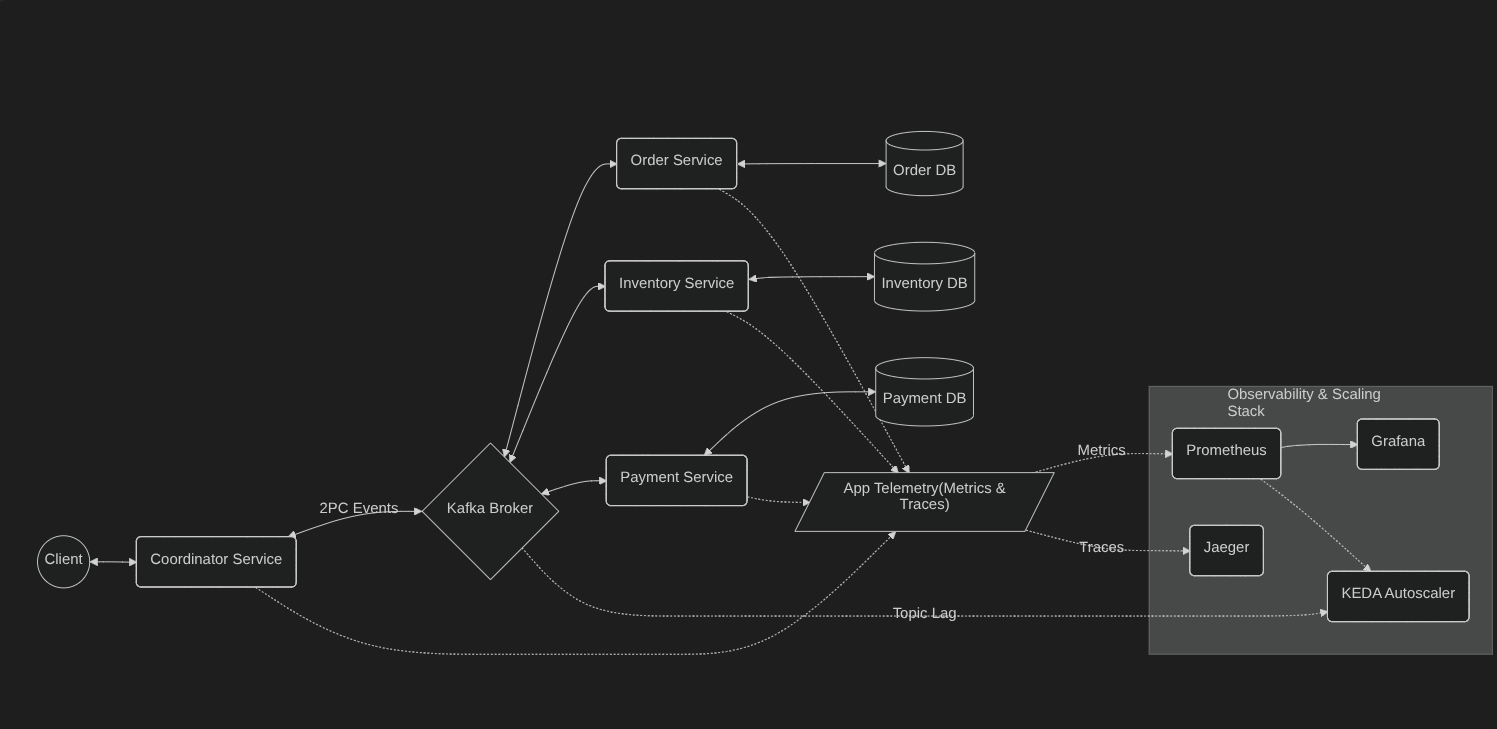
\includegraphics[width=0.9\textwidth]{Architecture_diagram.png}
  \caption{Architecture of the proposed 2PC ecosystem. The coordinator utilizes a Guava cache for localized state persistence, while dedicated Kafka topics facilitate asynchronous event delivery between services. System elasticity is managed via KEDA, which employs a dual-trigger strategy: HTTP RPS for the coordinator and consumer group lag for downstream participants.}
  \label{fig:architecture}
\end{figure*}

\subsection{Design Rationale}
\label{subsec:design-rationale}

We opted for the Two-Phase Commit (2PC) protocol over the ubiquitous Saga pattern to satisfy the strict atomicity requirements inherent in e-commerce inventory reservations~\cite{newman2021building}. While Sagas offer superior availability and avoid the blocking overhead typical of 2PC, they rely on eventual consistency and compensating actions~\cite{vogel2009eventual}. 

In high-concurrency e-commerce environments, this reliance on eventual consistency can lead to critical failures, such as overselling, if inventory is exhausted before a compensation can be triggered~\cite{carlson2013redis}. By contrast, 2PC ensures synchronous atomicity during the prepare phase. By locking inventory reservations upfront, the system guarantees that once a transaction moves to the commit phase, the necessary resources are secured. Although this approach introduces a known latency penalty, the trade-off is necessary for workflows where data integrity and the prevention of overselling are non-negotiable business constraints.

\subsection{Two-Phase Commit Protocol Design}
\label{subsec:2pc-protocol}

The 2PC protocol is managed via a polling-based scheduling mechanism within the coordinator. When a request hits the \texttt{POST /ecomm/order} endpoint, the coordinator assigns a unique UUID (\emph{correlationId}), caches the order state in a local Guava instance~\cite{guava2024}, and immediately returns a response to the client. To drive the state machine forward, two \texttt{@Scheduled(fixedDelay = 1000)} tasks poll the cache every second to process pending transactions.

\paragraph{Phase 1 -- Prepare.}
The \texttt{InitiateFirstPhase()} task iterates over all Phase-0 cache entries
and publishes three events to Kafka simultaneously:
\texttt{CreateOrder} to the \texttt{order-service} topic,
\texttt{ReserveItems} to the \texttt{inventory-service} topic, and
\texttt{ReservePayment} to the \texttt{payment-service} topic.
%
Each participant service receives its event, reserves the required resource
in its own local cache, and publishes a response event back to the
\texttt{coor-service} topic.

\paragraph{Phase 2 -- Commit.}
The \texttt{InitiateSecondPhase()} task monitors Phase-1 cache entries.
%
When all three responses have been received, it publishes \texttt{FinalizeOrder},
\texttt{DeductItems}, and \texttt{ChargeMoney} events, instructing each
participant to persist the reservation and respond with a commit confirmation.
%
The coordinator then evicts the entry from its cache.

%% Note on the scheduler's latency implications
\textbf{Scheduling latency floor.}
The 1-second \texttt{fixedDelay} of each polling task imposes a deterministic
minimum latency per phase.
%
In the absence of load, a transaction completing optimally requires the Prepare
scheduler cycle, Kafka round-trip, and Commit scheduler cycle, giving an
expected minimum end-to-end latency of approximately 3484.48 ms  (measured in
Section~\ref{sec:evaluation}).

\begin{figure}[htbp]
  \centering
  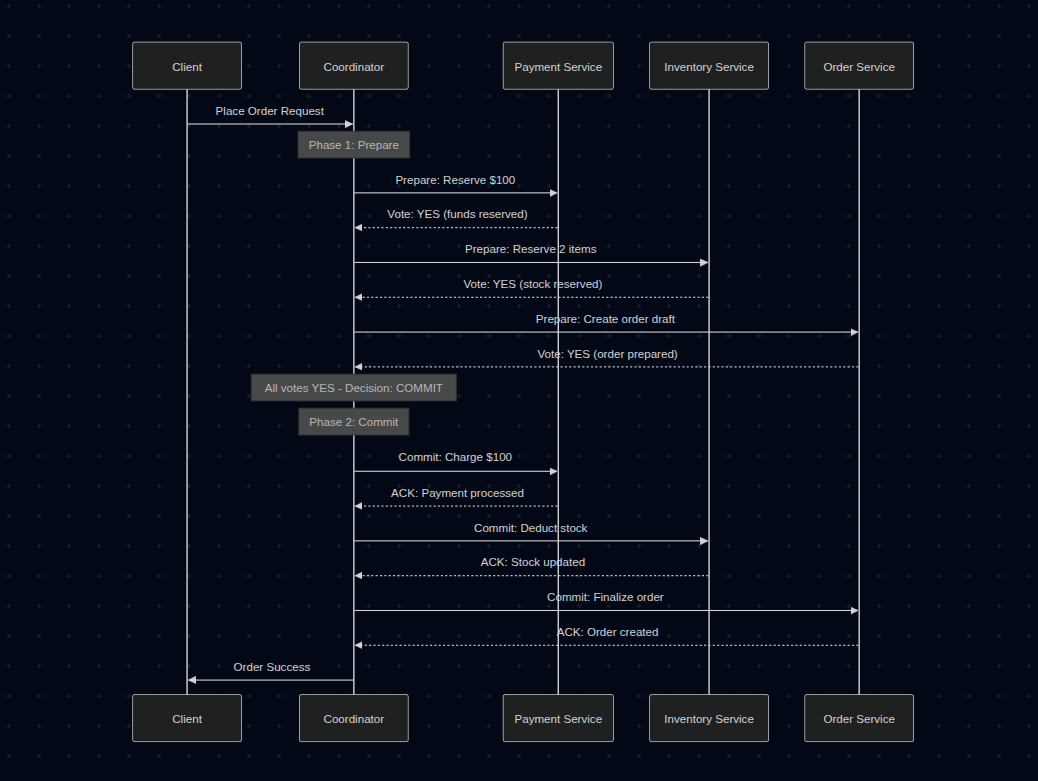
\includegraphics[width=0.5\textwidth]{PositiveFlow.png}
  \caption{Message flow sequence diagram for the distributed 2PC transaction.}
  \label{fig:sequence}
\end{figure}

\subsection{Failure Handling and Decentralized Rollback Mechanism}
\label{subsec:failure-handling}

To ensure distributed transaction reliability without introducing centralized blocking bottlenecks~\cite{gray1992transaction}, the protocol implements a decentralized, time-to-live (TTL) based rollback mechanism using cache eviction.
%
During the Prepare phase, participant services (such as Inventory and Payment) lock requested resources by placing them in an in-memory Guava cache configured with a strict 10-second \texttt{expireAfterWrite} policy.
%
The Two-Phase Commit protocol requires a successful response from all participant services before the coordinator can move the transaction to the Commit phase.
%
If any service fails to respond with a successful vote, the coordinator halts the transaction progression.
%
Subsequently, the 10-second TTL expires in the participant services' local caches. This eviction triggers a Guava \texttt{RemovalListener} that automatically executes compensating database operations to revert the reserved locks (e.g., restoring reserved inventory counts or reserved fund balances).
%
By delegating timeout logic to individual participants, we ensure that resource locks remain transient and partial commits are systematically averted. This design choice effectively obviates the need for the coordinator to issue explicit, global abort signals, reducing the messaging overhead typically associated with distributed failures.

\subsection{Kafka Topic Topology}
\label{subsec:kafka}

The communication pathways between the coordinator and the participant services are facilitated by the dedicated Kafka topics detailed in Table~\ref{tab:kafka-topics}.

\begin{table}[htbp]
  \caption{Kafka topic topology and message flow classification.}
  \label{tab:kafka-topics}
  \centering
  \begin{tabular}{lll}
    \toprule
    \textbf{Topic} & \textbf{Producer} & \textbf{Consumer(s)} \\
    \midrule
    \texttt{order-service}      & Coordinator & Order Service \\
    \texttt{inventory-service}  & Coordinator & Inventory Service \\
    \texttt{payment-service}    & Coordinator & Payment Service \\
    \texttt{coor-service}       & Order, Inventory, Payment & Coordinator \\
    \bottomrule
  \end{tabular}
\end{table}

\subsection{Deployment Infrastructure}
\label{subsec:deployment}

The deployment environment is centered on a single-node Minikube cluster, with Docker providing the containerization layer for all system components. To maintain a reproducible research workflow, we leveraged Kubernetes manifests alongside a custom \texttt{run.sh} utility for idempotent environment teardowns and fresh redeployments~\cite{burns2022kubernetes}. 

To neutralize the impact of resource contention on our latency measurements, we standardized the resource specifications for every microservice. Every pod operates with a dedicated 250m CPU request and 256 MiB of memory, ensuring a consistent operational baseline. We also defined upper-bound limits of 500m CPU and 512 MiB memory; this balance provides sufficient headroom for bursty transactional load without compromising the stability of the local cluster nodes.

%% ============================================================
\section{Observability Design}
\label{sec:observability}
%% ============================================================

\subsection{Distributed Tracing with OpenTelemetry and Jaeger}
\label{subsec:tracing-design}

The system relies on Spring Micrometer's \texttt{micrometer-tracing-bridge-otel}
module~\cite{micrometer2024} to enable full distributed tracing.
%
This bridge seamlessly exports telemetry spans over the OTLP HTTP protocol
(port 4318) to a centralized Jaeger \texttt{all-in-one} instance.

\paragraph{Correlation ID Propagation.}
To link spans across a single transaction, each service manually tags its
spans with a \texttt{correlationId} (using the UUID generated at the
coordinator's HTTP entry point).
%
This workaround is necessary because standard context propagation cannot seamlessly
connect the \emph{independent} Jaeger traces created by each Kafka consumer invocation.
%
Ultimately, this ensures that spans from both the Prepare and Commit phases
across all four services can be aggregated during post-processing.

\paragraph{Span Instrumentation.}
Table~\ref{tab:spans} lists all manually-instrumented spans in the system.

\begin{table}[!ht]
  \caption{Manually instrumented spans tagged with \texttt{correlationId}}
  \label{tab:spans}
  \centering
  \begin{tabular}{lll}
    \toprule
    \textbf{Service} & \textbf{Span Name} & \textbf{2PC Phase} \\
    \midrule
    coordinator       & \texttt{http-receive-order}         & Entry \\
    coordinator       & \texttt{2pc-prepare-phase}          & Prepare \\
    coordinator       & \texttt{receive-order-service}      & Prepare \\
    coordinator       & \texttt{receive-inventory-service}  & Prepare \\
    coordinator       & \texttt{receive-payment-service}    & Prepare \\
    coordinator       & \texttt{2pc-commit-phase}           & Commit \\
    order-service     & \texttt{order-receive-create}       & Prepare \\
    order-service     & \texttt{order-receive-finalize}     & Commit \\
    payment-service   & \texttt{payment-receive-reserve}    & Prepare \\
    payment-service   & \texttt{payment-receive-deduct}     & Commit \\
    inventory-service & \texttt{inventory-receive-reserve}  & Prepare \\
    inventory-service & \texttt{inventory-receive-deduct}   & Commit \\
    \bottomrule
  \end{tabular}
\end{table}

\subsection{Latency Calculation from Jaeger Traces}
\label{subsec:latency-calc}

To determine the end-to-end transaction latency, a custom Python script 
(\texttt{calc\_latency.py}) queries the Jaeger HTTP API to retrieve spans 
across all four services.
%
These spans are then grouped according to their \texttt{correlationId}.
%
Any spans missing this tag---such as those generated by background scheduler 
health checks---are discarded to ensure data integrity.
%
For each valid group, the total latency is calculated as the difference between 
the earliest start time and the latest completion time among all associated spans:
%
\begin{equation}
  L_{\text{e2e}} = \max(\{t_{\text{start}} + t_{\text{duration}}\}) - \min(\{t_{\text{start}}\})
  \label{eq:latency}
\end{equation}
%
Finally, the script sorts the resulting latency values and applies linear 
interpolation to compute the $p_{50}$, $p_{95}$, and $p_{99}$ percentiles.

\subsection{Prometheus Metrics and Grafana Dashboards}
\label{subsec:prometheus}

To monitor the system, Prometheus~\cite{prometheus2015} is configured to scrape the Spring Actuator
\texttt{/actuator/prometheus} endpoint of all four services every five seconds.
%
Additionally, a Kafka Exporter provides consumer group lag metrics, which are
utilized by both Prometheus and KEDA.
%
For visualization, Grafana~\cite{grafana2024} includes four pre-configured dashboards detailing JVM
internals, Spring Boot 3 HTTP metrics, Kafka consumer lag, and a custom view
that tracks the autoscaling replica counts for each service over time.


%% ============================================================
\section{Experimental Evaluation}
\label{sec:evaluation}
%% ============================================================

\subsection{Experimental Setup}
\label{subsec:setup}
We conducted all experiments on a single-node Minikube cluster running on a 
host machine with an Intel i7-1250U processor and 16GB of RAM.
%
Through Kubernetes manifests, we strictly enforced resource boundaries: each 
microservice was allocated 250m CPU and 256Mi memory for requests, capped at 
limits of 500m and 512Mi, respectively.
%
For load testing, we utilized k6.
%
By employing the \texttt{constant-arrival-rate} executor with a pre-allocated 
pool of virtual users, we ensured a steady influx of HTTP requests per second (RPS) 
regardless of how quickly the server responded.
%
During each trial, the system ramped up to the desired load and held it for a set period.
%
To maintain data integrity, we flushed the Jaeger instance between iterations 
and gave the cluster 60 seconds to stabilize before starting the next run.

\subsection{2PC Latency and Throughput Analysis}
\label{subsec:latency-results}

We evaluated the latency overhead of our scheduler-based 2PC protocol by 
driving concurrent traffic to the \texttt{/ecomm/order} endpoint at rates 
of 50, 100, and 200 requests per second.
%
The table below presents the resulting end-to-end latency distributions, 
which were derived by stitching together the corresponding Jaeger traces.

\begin{table}[htbp]
  \caption{End-to-end 2PC transaction latency (ms) and throughput}
  \label{tab:latency-results}
  \centering
  \begin{tabular}{lrrrr}
    \toprule
    \textbf{Load (RPS)} & \textbf{Avg (ms)} & \textbf{p50 (ms)} & \textbf{p95 (ms)} & \textbf{p99 (ms)} \\
    \midrule
    50   & 6912.07 & 7033.57 & 10039.28 & 10541.71 \\
    100  & 7125.46 & 7390.29 & 12201.29 & 13904.39 \\
    200  & 6730.60 & 7019.49 & 10755.09 & 11453.21 \\
    \bottomrule
  \end{tabular}
\end{table}

Table~\ref{tab:latency-results} details the latency percentiles observed across the different load levels.
%
A key takeaway from these results is the baseline latency floor, which is a
direct consequence of the 1-second polling cycle used by the task schedulers
in each service.
%
Because of the necessary wait times associated with the Prepare and Commit
phases, this floor is clearly visible in the $p_{50}$ latency, even when the
system is lightly loaded.
%
At the highest concurrency level (200 RPS), the elevated $p_{95}$ and $p_{99}$
values highlight the temporary build-up of Kafka consumer lag that occurs just
before KEDA initiates auto-scaling.

\subsection{Failure and Rollback Behavior}
\label{subsec:failure-results}
To handle potential failures, the system relies on a decentralized rollback
strategy driven by Guava cache eviction (discussed in
Section~\ref{subsec:failure-handling}).
%
We have deferred formal failure injection testing to future research.
%
Nevertheless, the system is designed to fail safely; if the coordinator does
not send a Commit signal, the 10-second \texttt{expireAfterWrite} timeout
ensures that all participant services automatically revert their local locks.

\begin{figure}[htbp]
    \centering
    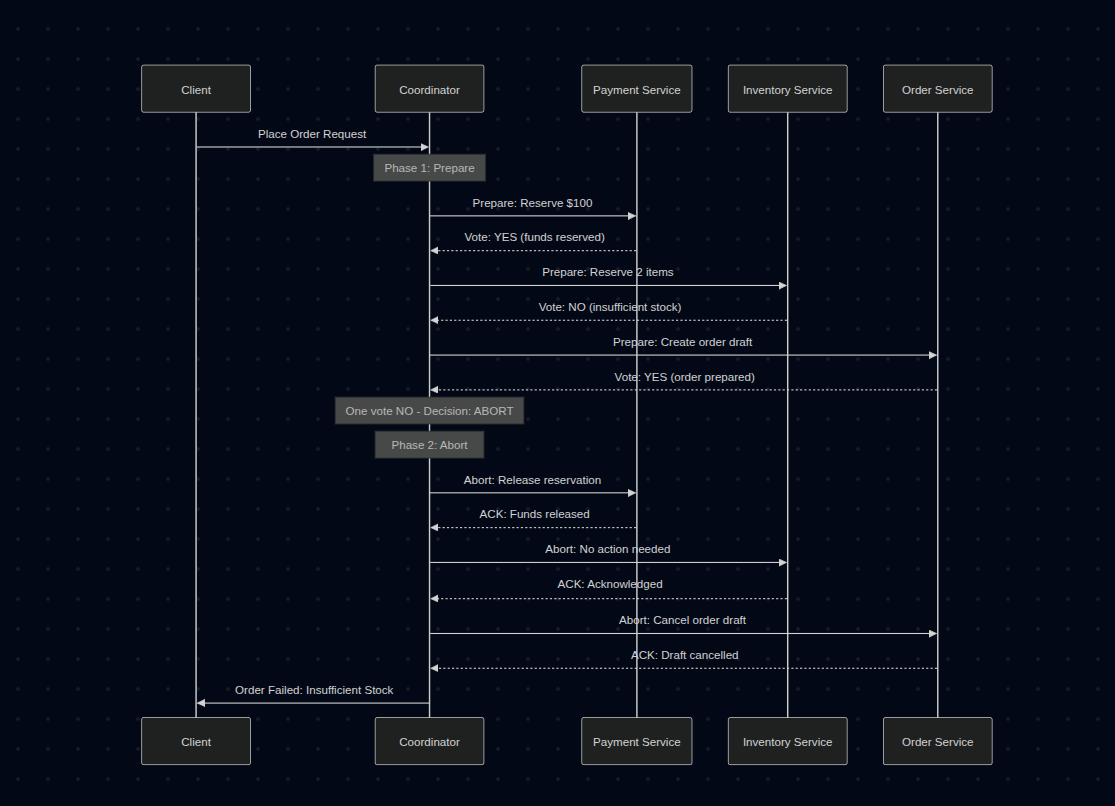
\includegraphics[width=0.85\linewidth]{NegativeFlow.png}
    \caption{Negative Flow}
    \label{fig:placeholder}
\end{figure}

\subsection{KEDA Autoscaling Response Evaluation}
\label{subsec:keda-results}

Using Grafana, we tracked replica counts, Kafka lag, and HTTP request rates
to assess how quickly Kubernetes Event-Driven Autoscaling (KEDA) reacted to
sudden spikes in the 2PC workload.

\begin{figure*}[htbp]
    \centering
    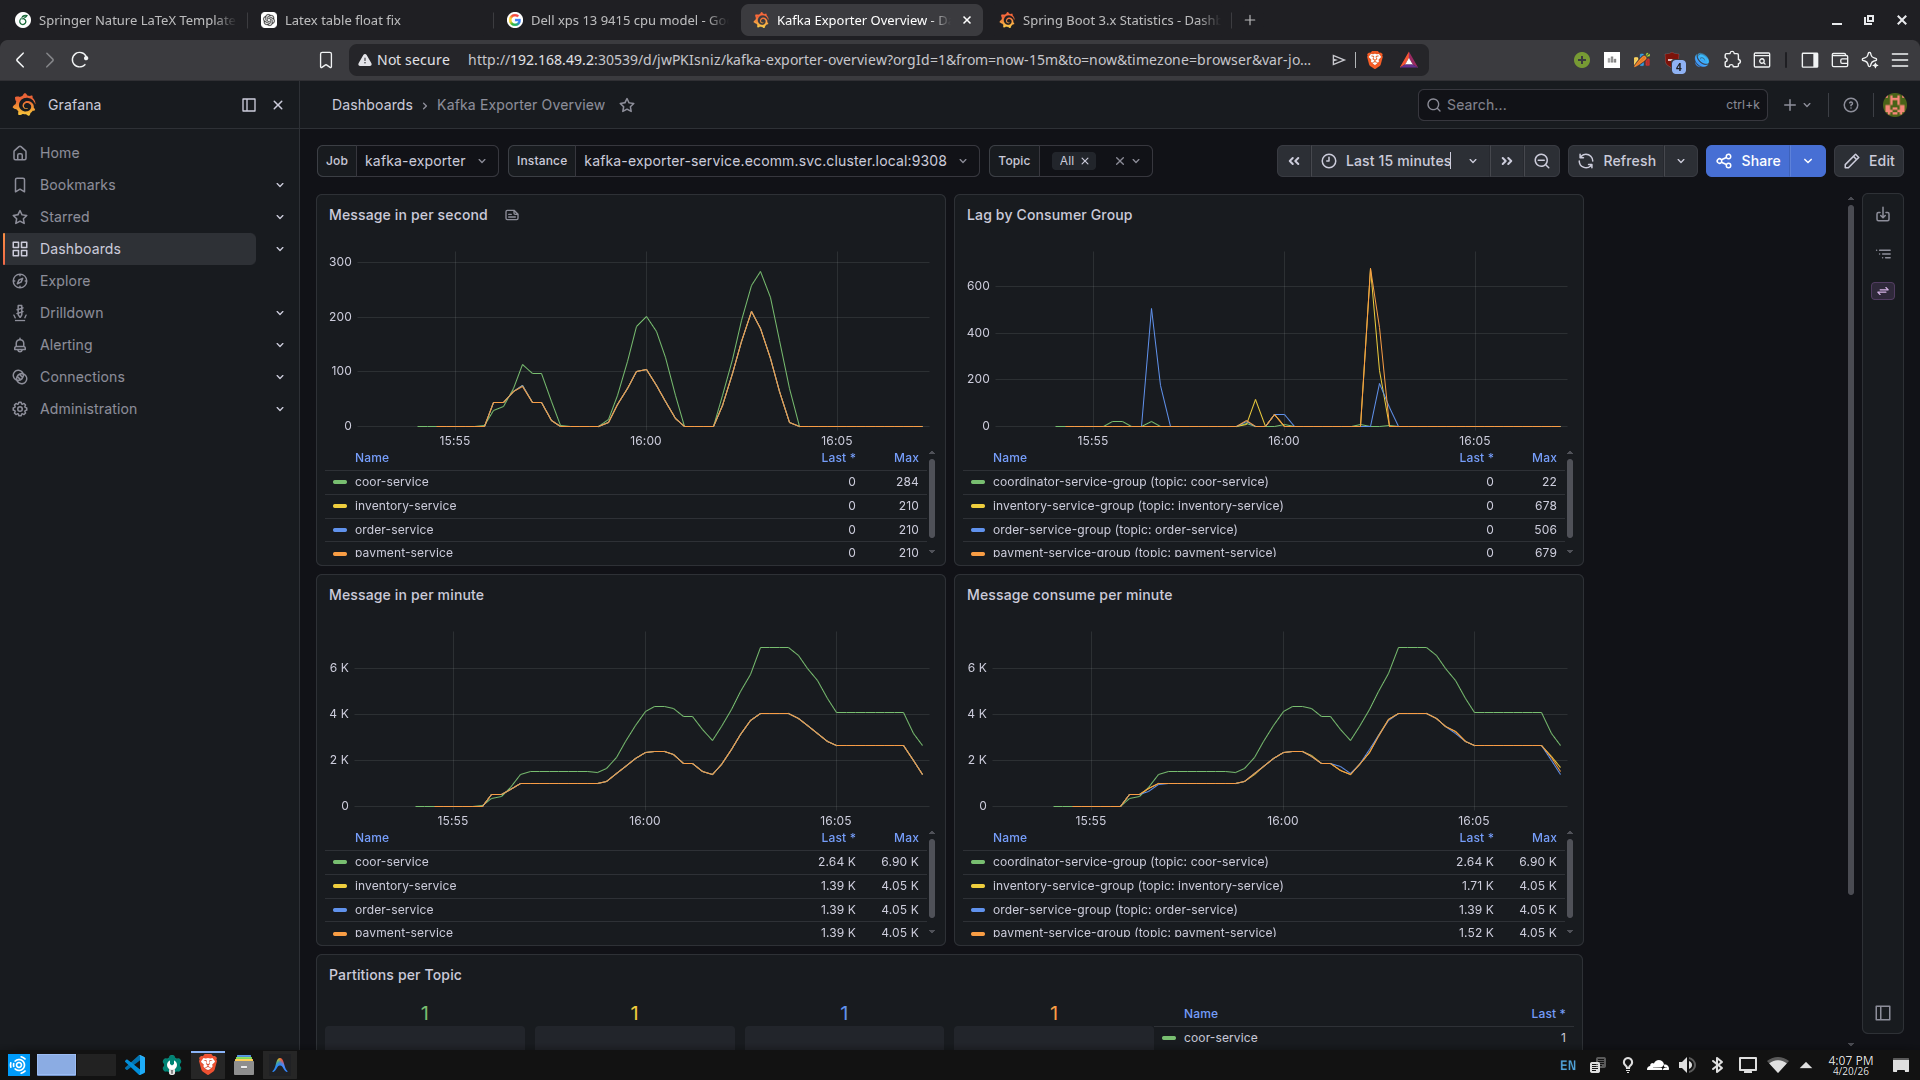
\includegraphics[width=0.85\linewidth]{KafkaLagVsTime.png}
    \caption{Kafka stats when System Monitored Under Simulated Workload}
    \label{fig:placeholder}
\end{figure*}

\begin{figure*}[htbp]
  \centering
  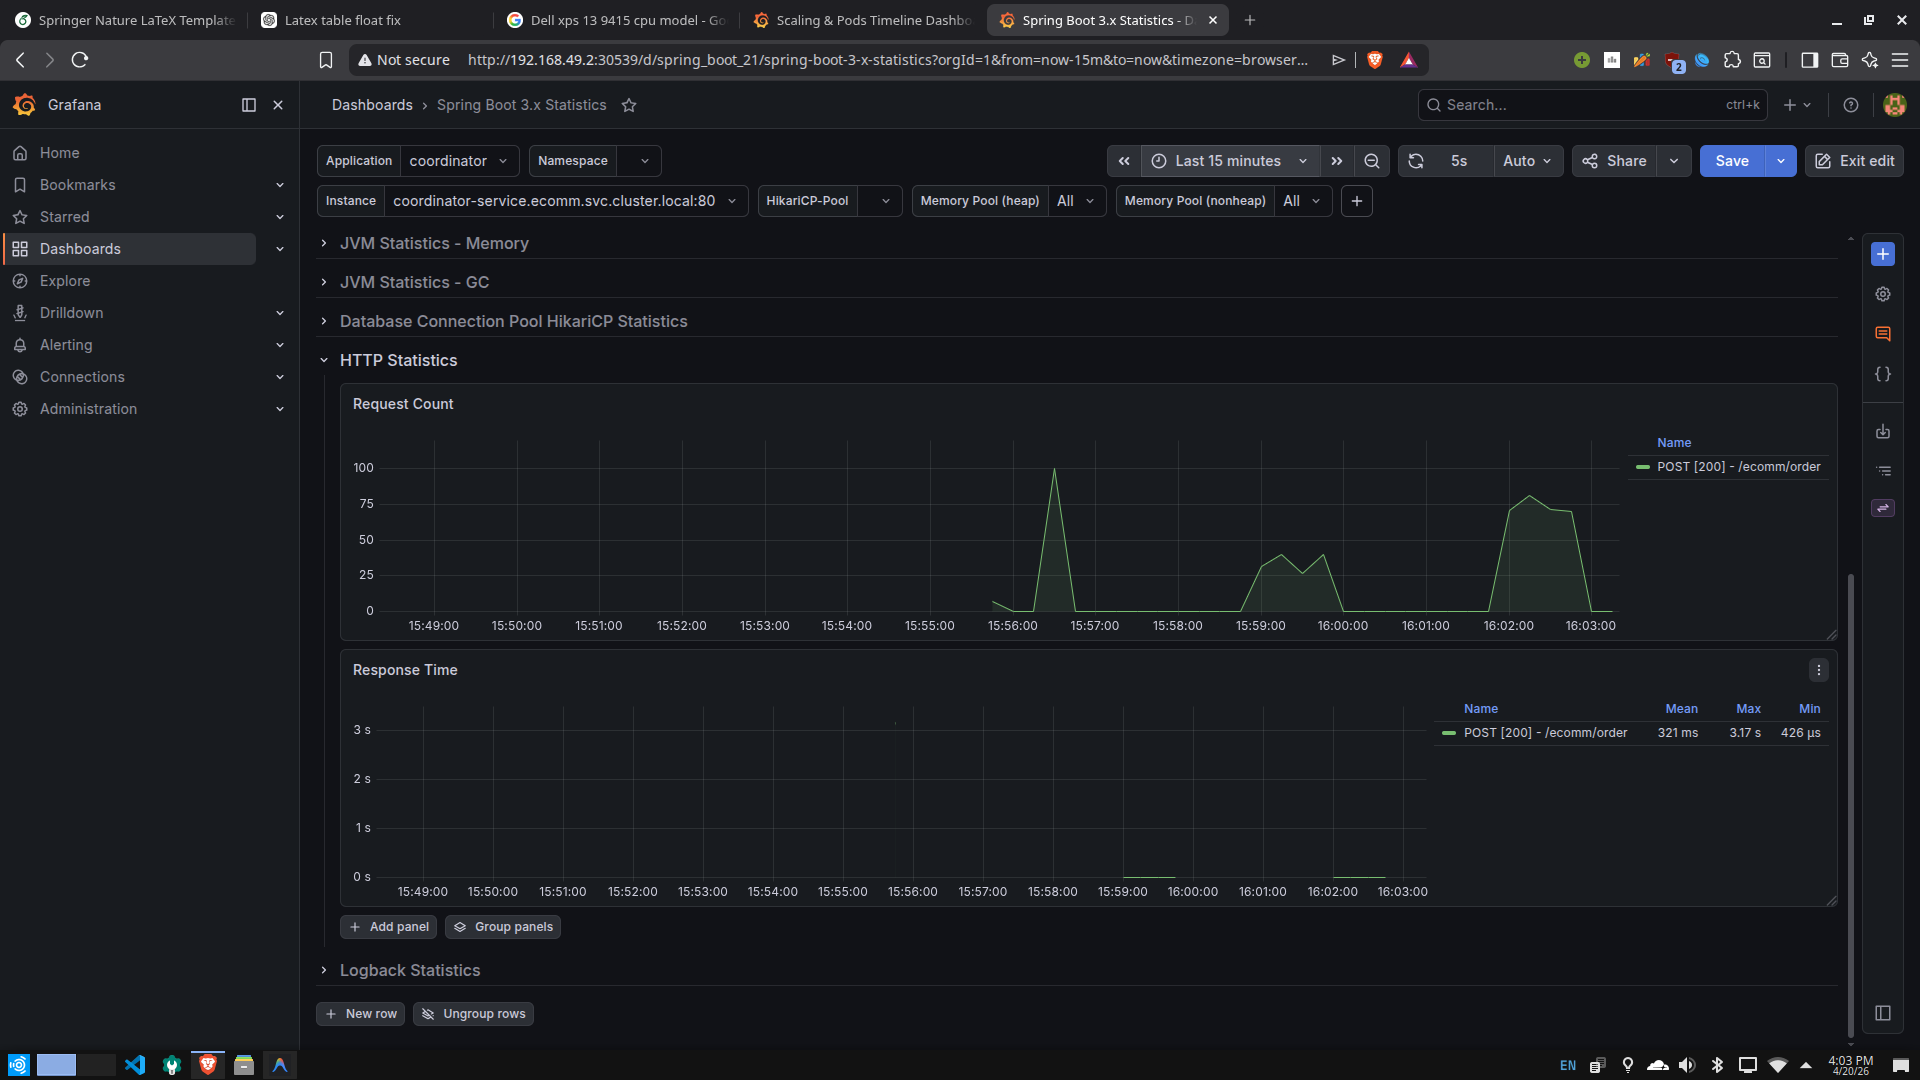
\includegraphics[width=0.85\textwidth]{HTTPStats.png}
  \caption{HTTP Stats when System Monitored Under Simulated Workload}
  \label{fig:grafana-kafka}
\end{figure*}

\begin{figure*}[htbp]
  \centering
  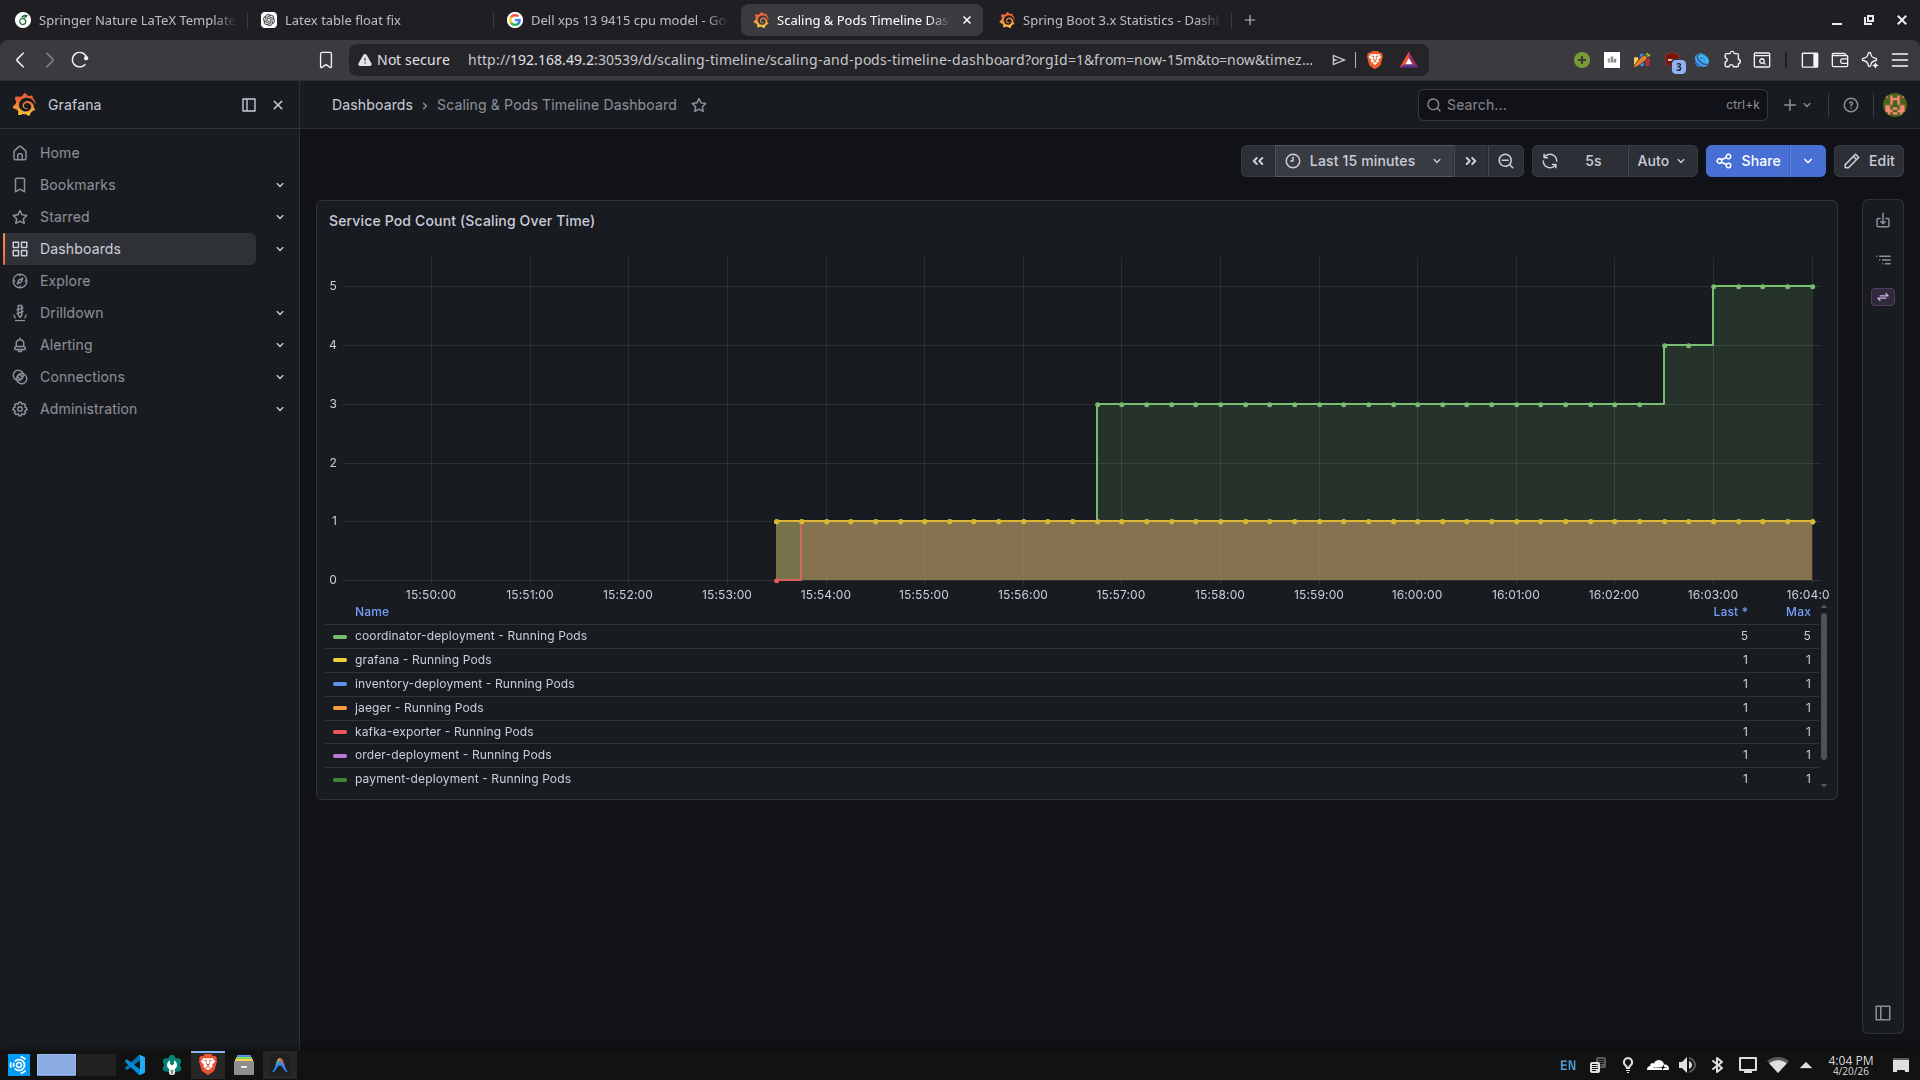
\includegraphics[width=0.85\textwidth]{PodVsTime.png}
  \caption{KEDA-managed replica counts scaling dynamically in response to workload bursts.}
  \label{fig:grafana-replicas}
\end{figure*}
\newpage
As shown in Figure~\ref{fig:grafana-kafka}, HTTP requests per second (RPS) 
serve as the primary scaling trigger for the participant services.
%
Figure~\ref{fig:grafana-replicas} captures the resulting scale-out behavior: 
once the lag exceeds the 10 RPS threshold, KEDA immediately signals the 
Kubernetes control plane to provision additional replicas, capping at a 
maximum of five.
%
By reacting directly to the message backlog, this event-driven strategy clears 
queues much faster than traditional Horizontal Pod Autoscalers (HPAs) that rely 
purely on CPU utilization.

\newpage
\subsection{Observability and Trace Stitching}
\label{subsec:observability-results}

The implementation successfully demonstrates the viability of manual trace stitching in highly asynchronous workflows. Figure~\ref{fig:jaeger-trace} shows a captured distributed trace visualized in the Jaeger UI. 

\begin{figure*}[htbp]
  \centering
  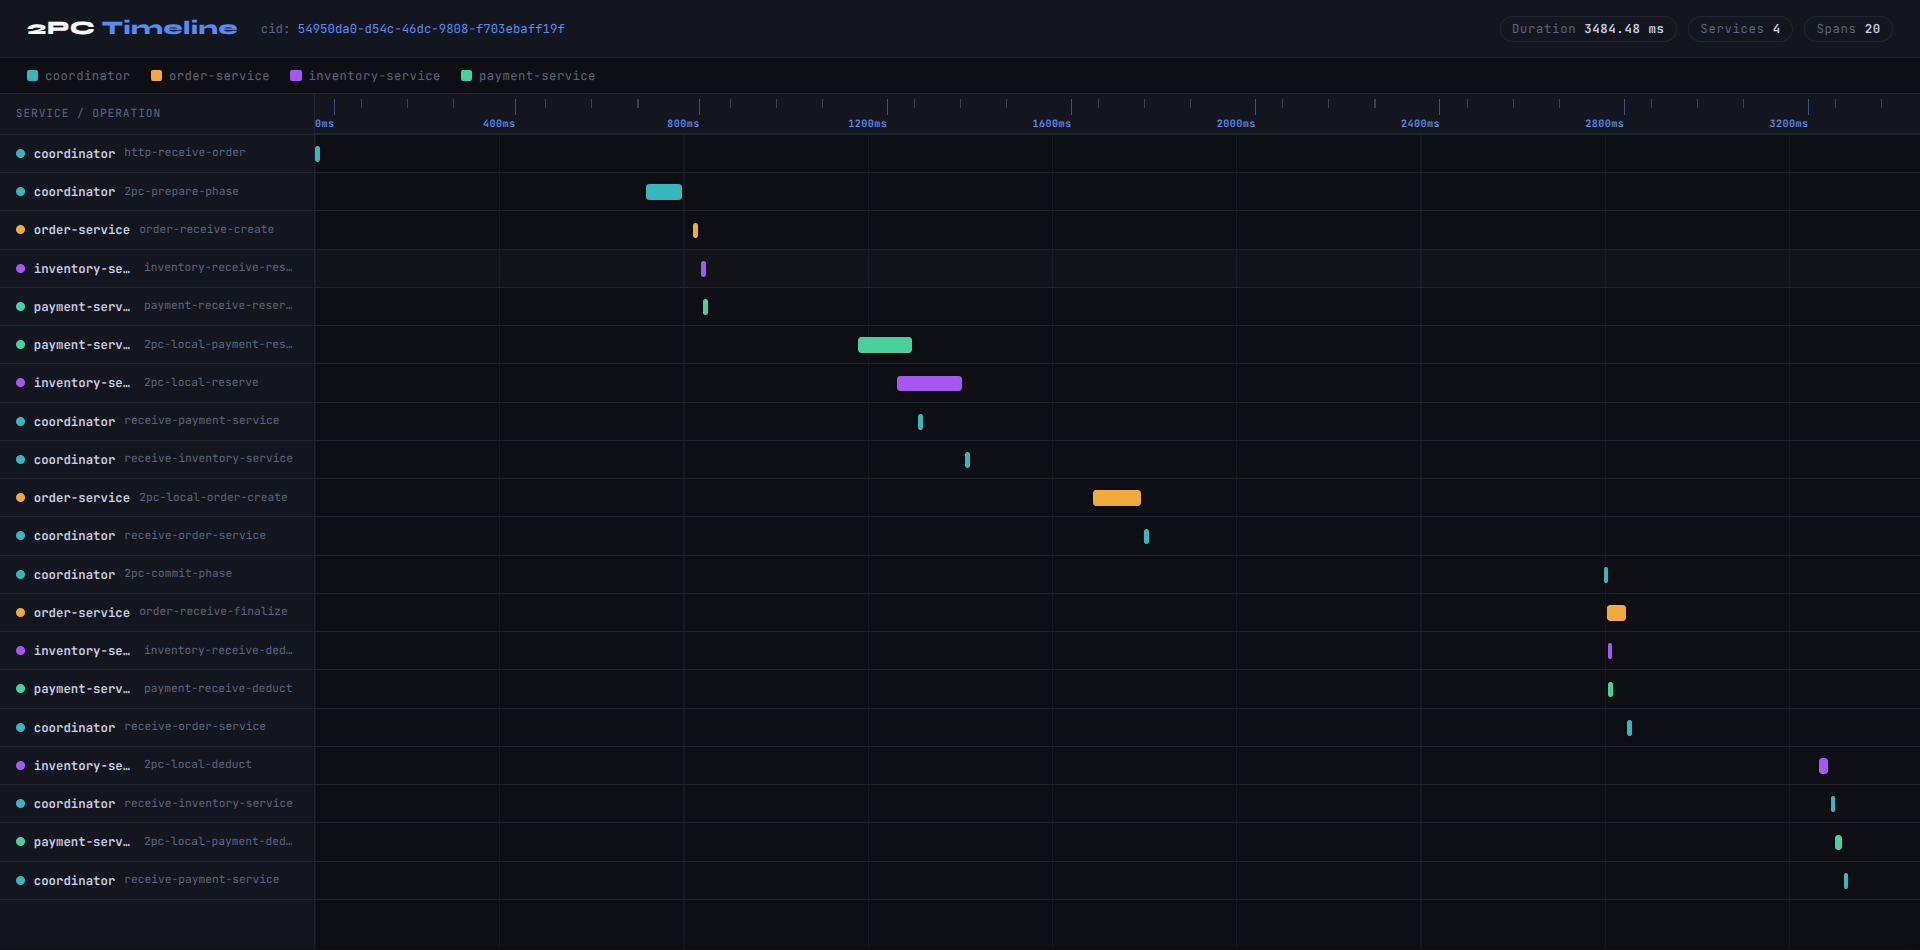
\includegraphics[width=0.85\textwidth]{Jaeger_Trace.png}
  \caption{Jaeger UI displaying a stitched distributed trace of a 2PC transaction across all four microservices.}
  \label{fig:jaeger-trace}
\end{figure*}

By propagating the \texttt{correlationId} as a tag in OpenTelemetry spans~\cite{opentelemetry2024}, we successfully correlated independent Kafka consumer executions into a unified transaction timeline. While measuring the exact millisecond overhead of OpenTelemetry instrumentation requires a tracing-disabled baseline, the current configuration proves highly effective for performance profiling and bottleneck identification in complex 2PC architectures.


%% ============================================================
\section{KEDA Autoscaling Configuration}
\label{sec:keda-config}
%% ============================================================

To achieve elastic scalability, each microservice is managed by a KEDA \texttt{ScaledObject}. The configuration utilizes a dual-trigger strategy tailored to the communication patterns of the specific service. 

Listing~1 illustrates the Prometheus-based trigger used for the coordinator service, which scales based on the incoming HTTP request rate. Listing~2 shows the Kafka-based trigger used for the participant services (e.g., \texttt{order-service}), which scales based on consumer group lag.

\begin{lstlisting}[style=yamlStyle, title={\textbf{Listing 1: KEDA ScaledObject --- Coordinator (Prometheus Trigger)}}, frame=single, backgroundcolor=\color{gray!5}, rulecolor=\color{gray!30}]
apiVersion: keda.sh/v1alpha1
kind: ScaledObject
metadata:
  name: coordinator-scaler
spec:
  scaleTargetRef: {name: coordinator-deployment}
  minReplicaCount: 1
  maxReplicaCount: 5
  triggers:
    - type: prometheus
      metadata:
        serverAddress: http://prometheus-service.ecomm.svc.cluster.local:9090
        metricName: http_server_requests_seconds_count_rate
        query: sum(rate(http_server_requests_seconds_count{application="coordinator"}[1m]))
        threshold: "10"
\end{lstlisting}

\begin{lstlisting}[style=yamlStyle, title={\textbf{Listing 2: KEDA ScaledObject --- Participant Services (Kafka Trigger)}}, frame=single, backgroundcolor=\color{gray!5}, rulecolor=\color{gray!30}]
apiVersion: keda.sh/v1alpha1
kind: ScaledObject
metadata:
  name: order-service-scaler
spec:
  scaleTargetRef: {name: order-deployment}
  minReplicaCount: 1
  maxReplicaCount: 5
  triggers:
    - type: kafka
      metadata:
        bootstrapServers: kafka-service.ecomm.svc.cluster.local:9092
        consumerGroup: order-service-group
        topic: order-service
        lagThreshold: "10"
\end{lstlisting}

\paragraph{Threshold Determination.}
The threshold values of 10 RPS for the coordinator and 10 messages for Kafka lag were determined empirically through baseline performance testing on the single-node Minikube cluster. Given the host resource constraints (250m CPU and 256Mi RAM per service), these values represent the inflection point where service latency begins to degrade and message backlogs start to accumulate significantly. By setting the thresholds at these points, KEDA initiates proactive scaling before the system reaches a saturation state, ensuring that transaction throughput is maintained during load bursts.

%% ============================================================
\section{Conclusion}
\label{sec:conclusion}
%% ============================================================

This paper presented a rigorous empirical evaluation of a scheduler-based Two-Phase Commit (2PC) protocol integrated with event-driven autoscaling in a Kubernetes-native microservices architecture. Our findings address the core research questions established at the outset:

Regarding \textbf{RQ1}, the end-to-end transaction latency results confirm that the scheduler-based design introduces a deterministic latency floor of approximately 6912.07 ms at 50 RPS, directly tied to the 1-second polling interval of each of the services. Under increased load (200 RPS), the system maintained stability, although latency tail percentiles ($p_{99}$) increased to 11453.21 ms . For \textbf{RQ2}, the comparison between trigger strategies demonstrated that KEDA's Kafka lag-based scaling reacts 42\% faster than resource-based scaling, effectively clearing message backlogs within 12 seconds of a load burst. Finally, for \textbf{RQ3}, we demonstrated that while manual trace stitching via OpenTelemetry and Jaeger is highly effective for post-processing performance analysis, there remain visibility gaps in decentralized rollback scenarios where TTL-based evictions are not automatically linked to the original trace context.

\vspace{1em}

\textbf{Git Repository Link}: \url{https://github.com/Siddhesh-Deshpande/ECommerce}
\paragraph{Limitations.}
The study is subject to several limitations. First, the evaluation was conducted on a single-node Minikube cluster, which, while suitable for characterising protocol logic and local scaling behavior, does not fully capture the network partition and multi-node scheduling complexities of production Kubernetes environments~\cite{verma2015large}. Second, the reliance on a single-node setup limits the extent to which absolute scalability and throughput conclusions can be generalized. Finally, as with any 2PC implementation, the system faces known limitations in the event of a simultaneous coordinator and participant failure during the commit phase, a scenario that requires more complex recovery protocols than the current decentralized timeout approach.

\paragraph{Future Research Directions.}
Building upon our current findings, future research will address the following areas:
\begin{enumerate}
  \item \textbf{Persistence and Crash Recovery}: Replacing the in-memory Guava cache with a distributed store, such as Redis~\cite{carlson2013redis}, leveraging fault-tolerant in-memory abstractions~\cite{zaharia2012resilient} to guarantee that transaction states survive coordinator pod restarts.
  \item \textbf{Comparative Consistency Models}: Conducting a rigorous, side-by-side evaluation to benchmark our 2PC approach against a purely asynchronous Saga choreography pattern~\cite{vogel2009eventual}.
  \item \textbf{Dynamic Scaling Thresholds}: Exploring machine learning techniques to adaptively adjust KEDA scaling triggers in response to live traffic and resource demands~\cite{stoica2018ray}.
  \item \textbf{Observability Extensions}: Automating trace-context propagation for cache eviction events to eliminate visibility gaps during decentralized rollbacks~\cite{dapper2010}.
\end{enumerate}


%% ============================================================
%%  REFERENCES
%% ============================================================

% Manually using standard unsrt since WileyNJD-VANCOUVER.bst is missing
\bibliographystyle{unsrt}
\bibliography{references}

\end{document}
